\documentclass{ds-report}
\assignment{Java EE} % Set to `Java RMI`, `Java EE` or `Google App Engine`.
\authorOne{Dries Janse} % Name of first team partner.
\studentnumberOne{r0627054} % Student number of first team partner.
\authorTwo{Steven Ghekiere} % Name of second team partner.
\studentnumberTwo{r0626062}  % Student number of second team partner.
\usepackage{graphicx}

\begin{document}
	\maketitle

	\paragraph{1. Outline the different tiers of your application, and indicate where classes are located.} \mbox{}\\\\
The different tiers of the application are visualized in figure \ref{fig:tier_diagram}.
Our application has 3 main tiers: The application machine, the business tier and the enterprise information system tier. The only classes which aren't specified are the classes in the carRental-lib project. It contains the following classes: CarType, Quote, Reservation, ReservationConstraints, ReservationException, CarRentalSessionRemote, ManagerSessionRemote. These classes are packaged in a jar and both the client and ejb project uses them.

	
	\paragraph{2. Why are client and manager session beans stateful and stateless respectively?} \mbox{}\\\\
Both the manager and client session beans are server-side (EJB) Enterprise Java Bean components. The component is a session bean, because it represents a session with the client.
The client session is a stateful session bean, this means that it retains state between method invocations. The (conversational) state consists of the values of the instance variables. The client session is stateful because it keeps the conversational state, it contains the name of the renter and the list of quotes of this renter.
The manager session is a stateless session bean, this means that it does not retains the conversational state. In our application there is no need to make the manager session stateful because all instances of the bean are equivalent. This allows the EJB container to assign an instance to any manager.



	\paragraph{3. How does dependency injection compare to the RMI registry of the RMI assignment?} \mbox{}\\\\
The RMI registry of the RMI assignment is a simplified name service that allows clients to get a reference to a remote object. The @EJB annotation can be applied on fields or methods to inject dependencies. The EJB client container will first perform a JNDI lookup to locate the dependency. JNDI stands for Java Naming and Directory Interface, it allows distributed application to look up services in an abstract way.
With JEE we don't have to explicitly instantiate, with the "new" keyword, the objects of which we need a reference. JEE provides these injection mechanisms. We only have to declare the needed resources with the annotations (@EJB) that denotes the injection point to the compiler. The container will then provide an instance of the required resource at runtime. The advantage of using dependency injection is that it simplifies our code because the container automatically provides these instances.


\clearpage



	\paragraph{4. JPQL persistence queries without application logic are the recommended approach for retrieving rental statistics. Can you explain why this is more efficient?} \mbox{}\\\\
JPQL uses the entity object model instead of querying actual tables in the database. This makes it more easy for the Java developer. To answer on the question; there are multiple advantages of retrieving rental statistics without using application logic.\\\\
For example, retrieving the number of reservations made by a particular car renter. With only a JPQL query, one number is returned. Only one number is send from the database server back to the Jave EE Server. The JEE server then only has to create an integer and store the result. If we used application logic to calculate the number of reservations for a particular car renter, we first had to request all the reservations from the database. This results in a lot more network traffic between the database server and the Java EE Server. For each reservation an object is created on the Java EE server, which results in a big memory usage. The application now has to make operations on the list of reservations, which can take substantially longer than a database. This is because the database can be indexed.




	\paragraph{5. How does your solution compare with the Java RMI assignment in terms of resilience against server crashes?} \mbox{}\\\\
The resilience against server crashes depends on which component crashes on which server. This is because we are talking about a distributed application. In the Java RMI assignment all the car rental companies store their data in memory. So if a server crashes which contains a car rental company all the data is lost when the server reboots. If the server which contains the Naming Service component crashes and reboots, all the car rental company references are lost, this is because they are stored in memory. If the server with Rental Agency crashes and reboots all the sessions are lost with the client.\\
The biggest difference with this assignment is that all the data is stored in a database. So if the server crashes which contains the CarRentalSession and ManagerSession classes all the data will not be lost. Only the data of the sessions will be lost because they are not persistent. 


		\paragraph{6. How does the Java EE middleware reduce the effort of migrating to another database engine?} \mbox{}\\\\
The entities in the application are persisted in the same manner, the only change is the location and name of the database. The persistence unit (persistence.xml) stores all the information needed for migrating to another data source. It stores information such as the data source, table generation strategy, validation strategy, etc. We can specify that it automatically  generates the relations and the tables of the entities.  
For the actual migration to another database, the copying of the data from one database to another, is done by the database administrators. They have to set up a migration strategy for retrieving the database from the first database and inserting it into the new database. 

 

	\paragraph{7. How does your solution to concurrency prevent race conditions?} \mbox{}\\\\
The car rental session is a stateful session bean, this means that every user will get his own session scoped instance. The next thread will wait until the first thread finishes. One user cannot execute the same code in parallel, but different users can.
The manager session is a stateless session bean, this means that every thread will get a different instance of the EJB from the pool. The same code can be executed in parallel.\\\\\clearpage
Thread handling is done by EJB container. JSE level thread handling is discouraged to use by the developer before JEE 7. This means that, for example, the use of the 'synchronized' keyword is discouraged.\\\\
In our solution we made use of a transaction for confirming the quotes of a particular car renter. If not all the quotes could be confirmed than a roll back will happen and a reservation exception will be thrown. This happens when multiple renters try to confirm their quotes at the same time. For specifying the transaction we made use of the @TransactionAttribute annotation.



	\paragraph{8. How do transactions compare to synchronization in Java RMI in terms of the scalability of your application?} \mbox{}\\\\
Transactions make sure the required data modifications are either all saved (committed) or rolled back. If any of the statements fail of our transaction, the transaction will roll back and all the statements are undone. Since the EJB container handles the rollback, we do not need to implement the reverse operation. We only need to raise an exception or telling the container explicitly that something went wrong.\\\\
Within Java RMI we cannot make use of the rollback functions and thus we needed to implement the rollback functionality ourselves.\\\\
Transactions are better scalable, different operations can be executed on different data sources in parallel by different threads. This was not the case in the Java RMI assignment, we had to make the method or list synchronized. This means that only one thread can access the resource at a time. All other threads attempting to enter the synchronized block are blocked until the first thread inside the block exits. This makes the Java RMI less scalable in comparison with transactions.




	\paragraph{9. How do you ensure that only users that have specifically been assigned a manager role can open a ManagerSession and access the manager functionality?} \mbox{}\\\\
In our application we made use of the @RolesAllowed annotation. We specified the annotation at class level of the ManagerSession. By doing this it applies to all the methods in the class. In this annotation we only putted the Manager role. So every person or group which has the manager role assigned can use the methods.
On out GlassFish server we created a couple of persons with the manager role and we enabled the automatically mapping functionality. By doing this the users have to provide their username and password before executing the manager methods. 
	
	
	\paragraph{10.  Why would someone choose a Java EE solution over a regular Java SE application with Java RMI?} \mbox{}\\\\
The answer on this question can be found in the introduction of the first JEE assignment. Java EE is a middleware which adds services relevant for distributed systems to Java SE. It provides services as transactions, persistence and session management. This allows the developer to cleanly structure business logic, client interaction and back-end processing.
If someone would develop an enterprise-grade Java application, he would preferably use Java EE because it is a powerful model. It is also involved into frameworks such as Hibernate and Spring. It wouldn't be impossible to create a similar application using Java SE, but it would require a lot more work and would be less performant. 

	
\begin{figure}
  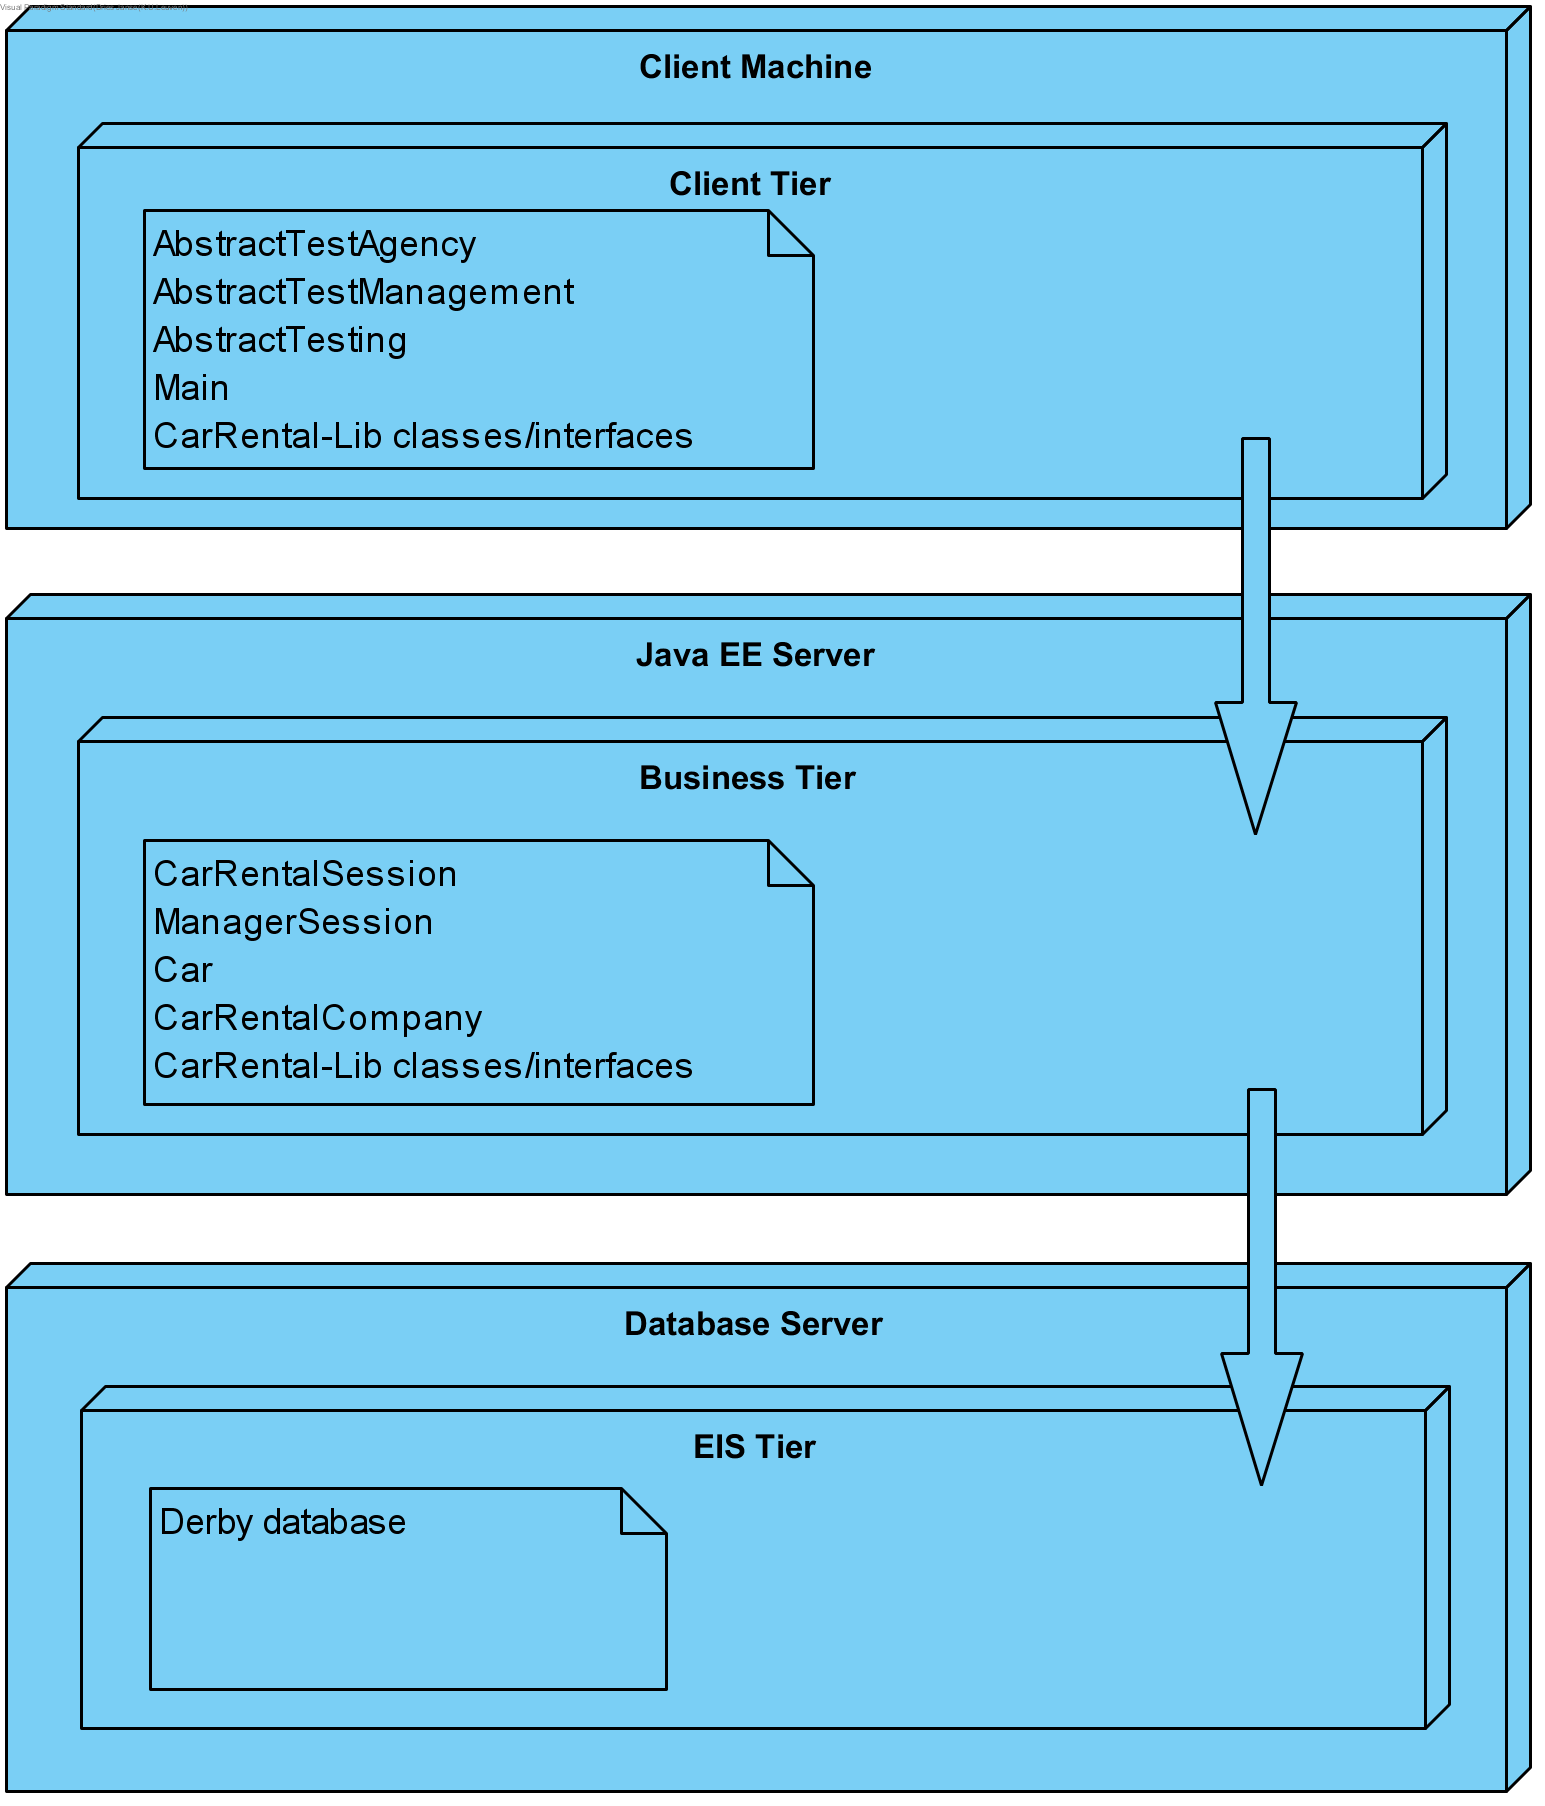
\includegraphics[width=\linewidth]{tier_diagram.png}
  \caption{Different tiers of the application}
  \label{fig:tier_diagram}
\end{figure}	
	
	\clearpage


	% You can include diagrams here.
	
\end{document}